\documentclass[a4paper, 12pt]{scrartcl}

\usepackage{amsmath}
\usepackage{tikz}
\usetikzlibrary{shapes.misc, calc}
%\usepackage{showframe}

\begin{document}
\title{Sujet de Grand Oral - Simulation de l'atterissage de Apollo 11 sur la Lune }
\author{Elliot Jullier}
\date{\today}
\maketitle

\pagenumbering{roman}
\tableofcontents

\newpage
\pagenumbering{arabic}




\section{- Etapes de l'Atterissage}
\subsection{- Parametres initiaux : Orbite Circulaire}
Nous cherchons à modeliser la mission de Apollo 11 du 20-21 Juillet 1969 comme exemple d'atterissage
de fusée sur la Lune car cela donne un modèle avec beaucoups de statistiques grace à sa sigificance 
historique. 
\\
Il y a deux capsules en orbite a $111\ km$ d'altitude au-dessus de la surface de la Lune. La \emph{Command and Service Module} - CSM,
partie qui reste en orbite avec l'astronaut Michael Collins, et le \emph{Lunar Module} - LM, avec Neil Armstrong et Edwin `Buzz' Aldrin.
En sachant que les deux parties attachés sont en orbite circulaire a une altitude de $111\ km$ on peut calculer
la vitesse initiale $\| \overrightarrow{v} \| = 1628.9\ m\cdot s^{-1}$. 

\subsection{- Transfer de Hohmann : Ellipse Intermédiaire}
On sépare ensuite les deux modules et on assure une séparation de au moins $10\ m$ puis on pointe
le moteur de la LM dans la direction du vecteur vitesse mais dans le sens opposé. On effectue un changement $\Delta \overrightarrow{v} = -21,6\ m\cdot s^{-1}$ 
ce qui met la fusée en une orbite elliptique avec un aposélene à la location du changement (à $111\ km$) et
avec un perisélene à 180° et une altitude de $15,2\ km$. 
\\
\begin{center}
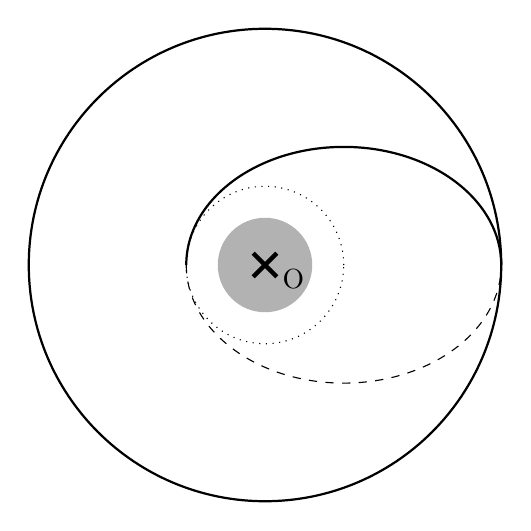
\begin{tikzpicture}
    \def \largeRadius {3}
    \def \smallRadius {1}
    \fill[black!30] (0,0) circle (0.2 * \largeRadius);
    \draw [ultra thick] (-0.05*\largeRadius,-0.05*\largeRadius) -- (0.05*\largeRadius,0.05*\largeRadius);
        \draw [ultra thick] (-0.05*\largeRadius, 0.05*\largeRadius) -- (0.05*\largeRadius,-0.05*\largeRadius);
        \node at (0.12*\largeRadius,-0.06*\largeRadius) {O};
    \draw[thick] (0,0) circle (\largeRadius);
    \draw[thick] ({(\largeRadius - \smallRadius)*0.5},0) + (0:{(\largeRadius + \smallRadius)*0.5} and 1.5) arc (0:180:{(\largeRadius + \smallRadius)*0.5} and 1.5);
    \draw[dashed] ({(\largeRadius - \smallRadius)*0.5},0) + (180:{(\largeRadius + \smallRadius)*0.5} and 1.5) arc (180:360:{(\largeRadius + \smallRadius)*0.5} and 1.5);
    \draw[dotted] (0,0) circle (\smallRadius);
\end{tikzpicture}
\\
\emph{Figure 1 - Transfer de Hohmann pour approcher la Lune}
\end{center}

\section{- La méchanique dans le modèle}
\subsection{- Implementation de la position, vitesse et acceleration}
\subsubsection{- Relations physique}
Dans le chapitre de la méchanique, on a vu la relation entre les vecteurs
de position, vitesse et acceleration:
\\

%\[\overrightarrow{OM} \begin{pmatrix} x \\ y \\ z \end{pmatrix}\]
%\[\overrightarrow{v} \begin{pmatrix} x' \\ y' \\ z' \end{pmatrix} = \frac{d \overrightarrow{OM}}{d t} \begin{pmatrix} x \\ y \\ z \end{pmatrix} \]
\[\overrightarrow{a} \begin{pmatrix} x'' \\ y'' \\ z'' \end{pmatrix}
= \frac{d\overrightarrow{v}}{d t} \begin{pmatrix} x' \\ y' \\ z' \end{pmatrix}
= \frac{d^2 \overrightarrow{OM}}{d t^2}\begin{pmatrix} x \\ y \\ z \end{pmatrix}\]
\\
\\
\subsubsection{- Implementation par approximation}
La manière dont on a implémenté cette relation dans le programme est d'approximer la 
continuité et l'evolution des vecteurs en les approximants en valeurs discretes. 
\\
Pour Unity le programme qu'on a utilisé pour la simulation, la valeur de temps entre chaque 'update' est de $\frac{1}{50}$ de seconde. 
\\
On calcule l'acceleration et on 'ajoute' ce vecteur a celui de la vitesse. Cela est comme faire: $v_{\text{future}} = v_{\text{courante}} + \Delta v$, cette action est répété
toute les $50^{\text{ième}}$ de seconde. On peut donc assimiler ajouter l'acceleration au vecteur vitesse comme ajoutant le $\Delta v$, 
les unités de l'acceleration en $m \cdot s^{-2}$ multiplié par des $s$ donne des $m \cdot s^{-1}$. En ajoutant le vecteur acceleration toute les $50^{\text{ième}}$ de seconde, 
on calcule le nouveau vecteur vitesse. 
\\
Similairement, pour la position, on prends la vitesse et on calcul la nouvelle position apres que la fusée
ait bougée pendant $\frac{1}{50}\ s$.

\subsection{- Evolution de l'acceleration}
Le moteur d'une fusée à un pourcentage de la 'puissance' maximale fourni une force
constante. 
\\
De plus:
\[F = ma \]
Par ailleur, le moteur d'une fusée brule la masse d'essence proportionellement a la 'puissance' fournie.
Cela a pour consequence que la fusée a une augmentation d'acceleration au fur et 
à mesure qu'elle utilise son carburant. 

\subsection{- Force Appliqués sur la Fusée}
\subsubsection{- Orbite Circulaire}
Dans une orbite circulaire uniforme, il y a seul la force de gravité qui agit sur la fusée.
On a:
\[ \overrightarrow{F} = \frac{GMm}{r^2}\overrightarrow{n} \Leftrightarrow \overrightarrow{a} = \frac{GM}{r^2}\overrightarrow{n}\]
Avec $G\text{ : la constante gravitationelle en } m^3 \cdot kg^{-1} \cdot s^{-2}\text{, } M \text{ : la masse de la Lune en } kg \text{, } 
\\ m \text{ : la masse de la fusée, } r \text{ : le rayon de l'orbite (} 
R_{\text{Lune}}\ +\ d_{\text{hauteur}} \text{), } \overrightarrow{n} \text{ : le vecteur unitaire} \\ \text{qui pointe vers le centre d'inertie de la Lune.}$
\\
De plus on est dans un mouvement circulaire donc: $\overrightarrow{a} = \frac{v^2}{r}\overrightarrow{n}$
\\
Ce qui donne:
\[\frac{v^2}{r}\overrightarrow{n} = \overrightarrow{a} = \frac{GM}{r^2}\overrightarrow{n} \Leftrightarrow 
v^2 = \frac{GM}{r} \Leftrightarrow v = \sqrt{\frac{GM}{r}}\]
Avec la direction de la vitesse étant tangantielle à la trajectoire circulaire à prendre.
\\
\\
\begin{center}
    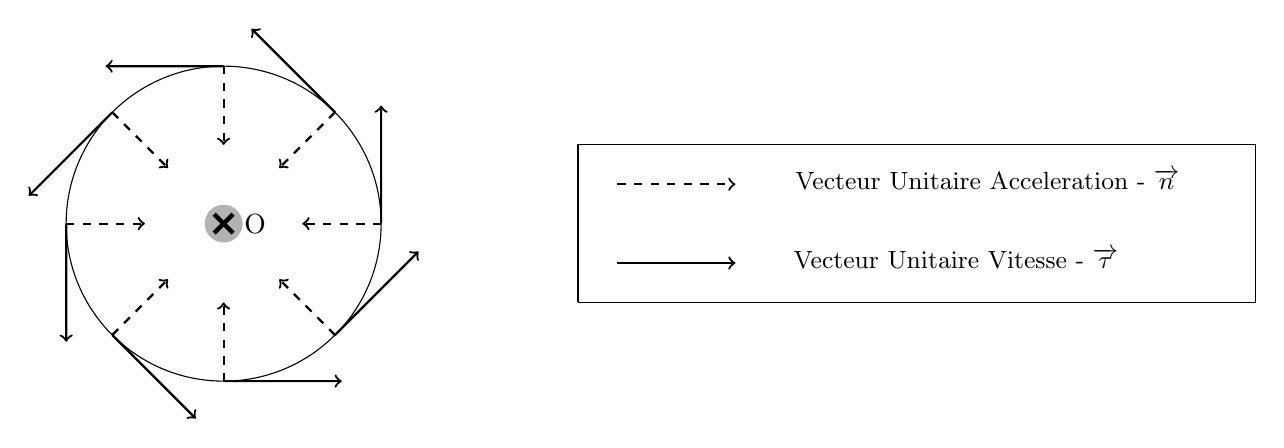
\begin{tikzpicture}
        \def \radius {2}; %cm
        \def \arrowLength {1.5}; %cm
        \def \innerArrowLength {1};
        \draw (0,0) circle (\radius);
        \fill[black!30] (0,0) circle (0.12*\radius);
        \draw [ultra thick] (-0.06*\radius,-0.06*\radius) -- (0.06*\radius,0.06*\radius);
        \draw [ultra thick] (-0.06*\radius, 0.06*\radius) -- (0.06*\radius,-0.06*\radius);
        \node at (0.2*\radius,0) {O};
        \foreach \a in {0,45,90,135,180,225,270,315}
            \draw [thick, ->] ({cos(\a)*\radius}, {sin(\a)*\radius}) -- ({cos(\a+atan(\arrowLength/\radius))*sqrt((\arrowLength)^2+(\radius)^2)},{sin(\a+atan(\arrowLength/\radius))*sqrt((\arrowLength)^2+(\radius)^2))});
        \foreach \a in {0,45,90,135,180,225,270,315}
            \draw [thick, dashed, ->] ({cos(\a)*\radius}, {sin(\a)*\radius}) -- ({(cos(\a+180)+cos(\a)*\radius)*\innerArrowLength},{(sin(\a+180)+sin(\a)*\radius)*\innerArrowLength});
        % Insert bos to right side with legende explaining the vecteurs vitesse and accelerations
        \draw [thick, dashed, ->] (5,0.5) -- (5 + \arrowLength, 0.5);
        \node at (5 + \arrowLength + 3.2, 0.56) {\small Vecteur Unitaire Acceleration - $\overrightarrow{n}$ \normalsize};
        \draw [thick, ->] (5,-0.5) -- (5 +\arrowLength,-0.5);
        \node at (5+ \arrowLength + 2.8, -0.44) {\small Vecteur Unitaire Vitesse - $\overrightarrow{\tau}$\normalsize};
        \draw (4.5, -1) -- (4.5,1) -- (11.6+\arrowLength,1) -- (11.6 + \arrowLength, -1) -- (4.5,-1);
    \end{tikzpicture}
    \\
    \emph{Figure 1 - Vecteurs Vitesses et Accelerations dans une Orbite Circulaire}
\end{center}







\end{document}